%\documentclass[11pt]{article}
\documentclass[a4paper,11pt,DIV=11]{article} % 

\usepackage[utf8]{inputenc}
\usepackage[english,ngerman]{babel}
\usepackage{amsmath}
\usepackage{amssymb}
\usepackage{mathtools}
\usepackage{fancybox}
\usepackage{color}
\usepackage{tikz}
\usetikzlibrary{arrows}
\usepackage{enumitem}

\usepackage{cite}
\usepackage{natbib}

\let\endtitlepage\relax

\newcommand{\n}{\nonumber}
\newcommand{\nn}{\nonumber\\}

\renewcommand{\refname}{Literatur}

\begin{document}
\begin{titlepage}
	\begin{figure}[h!]
	\centering
		\includegraphics[width=\textwidth]{images/thi_logo.png}
	\end{figure}
	
	\begin{center}
		\LARGE EMB$ ^2$\\ \large Vergleich zu OpenMP \\
		\vspace{1cm}
		\normalsize Simon Varga\\
		\normalsize 8. Juni 2015
	\end{center}
\end{titlepage}

%\tableofcontents{}

\section{Parallelisierung}
Wieso macht man das?
\begin{itemize}
	\item Multicore-Systeme
	\item möglichst schnelle Ausführung
\end{itemize}
Was kann ich parallelisieren?\footnote{siehe hierzu Beispiele aus dem Ordner "src" und in "workspace/Examples"}
\begin{itemize}
	\item Parallelen Anteil eines Programms
	\item Logisch unabhängige Programmteile
\end{itemize}
Was nun?
\begin{itemize}
	\item Programmstruktur identifizieren (Sequentieller $\leftrightarrow$ Paralleler Anteil)
	\item Geeignete Mittel einsetzen (Multithreading APIs)
	\item ggf. Anpassung ans Zielsystem (Optimierung auf X-Prozessoren)
\end{itemize}
Was kann ich einsetzen?
\begin{itemize}
	\item fork (erzeugt unabhängige Programme)
	\item PThread, std::thread, boost::thread, ...
	\item OpenMP
	\item EMB$ ^2$
\end{itemize}

\section{OpenMP}
\begin{itemize}
	\item Für C/C++, Fortran
	\item ähnlich mächtig zu PThreads 
	\item Präprozessormakros (\#pragma)
	\item integriert in Compiler
\end{itemize}
\section{EMB$ ^2$}
\begin{itemize}
	\item wird von Siemens entwickelt 
	\item aktuell Version 0.3.0 auf github\footnote{unter https://github.com/siemens/embb.git} OpenSource
	\item für Embedded (echtzeit) Systeme
	\item C/C++
	\item Abstraktion von (low-Level) Thread-Management
	\item Unterstützt Task Prioritäten
	\item Aufgebaut auf der MTAPI
\end{itemize}
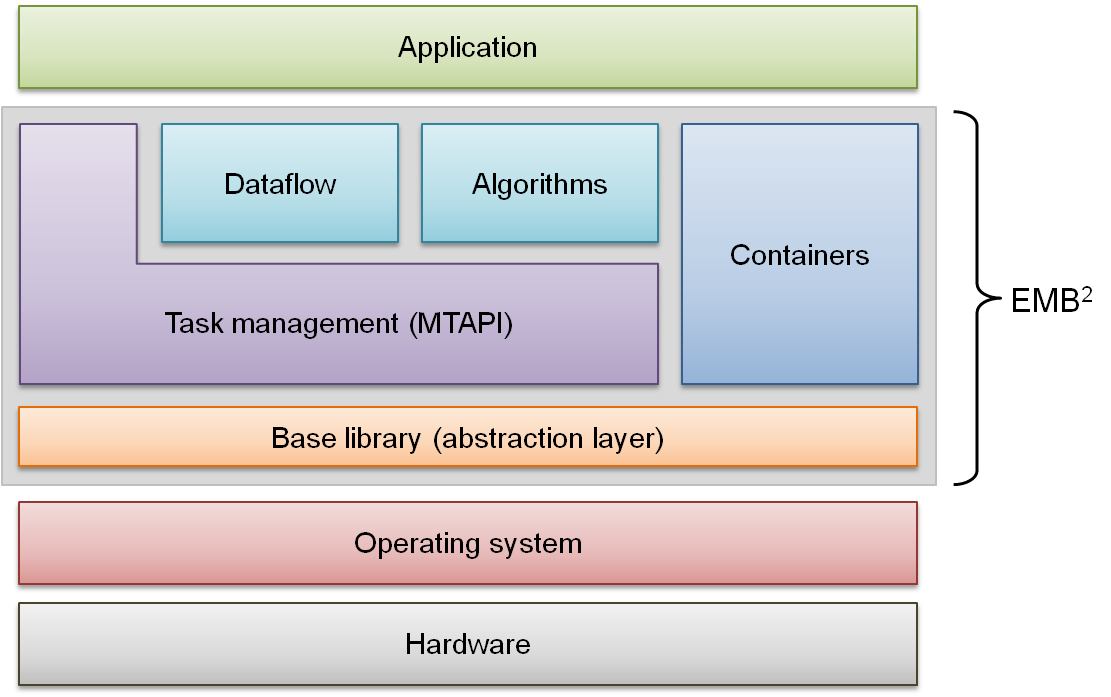
\includegraphics[width=\textwidth]{img/embb.png}
\section{Beispiele}
jeweils in einem Unterordner von "workspace"
\section{Ergebnis}
OpenMP
\begin{itemize}
	\item leicht zu schreiben
	\item vor allem für schon fertige Programme
\end{itemize}
EMB$ ^2$
\begin{itemize}
	\item für Echtzeitsystem, in denen 
	\begin{itemize}
		\item Timing eingehalten oder 
		\item Terminierung garantiert werden muss
	\end{itemize}	 	
	\item nur für neu geschriebene/durchdachte Programme
\end{itemize}

\end{document}